\chapter{Praktische Umsetzung}
    Im Folgenden werden wichtige Schritte der praktischen Umsetzung bei der Implementierung des Frameworks erklärt.

    Um die Umsetzung strukturiert zu gestalten,
    werden hierbei zuerst Planungsschritte aufgezeigt und
    im Anschluss daran die einzelnen Bestandteile nacheinander entwickelt,
    wobei jeweils zugehörige Unittests erstellt werden,
    um die korrekte Funktionalität sicherzustellen.

    \section{UML-Klassendiagramm}
        Das Klassendiagramm aus
        \vref{fig:Klassendiagramm} gibt die grundlegenden Klassen und
        Funktionen des Frameworks an.

        \begin{figure}[htp]
            \centering%
            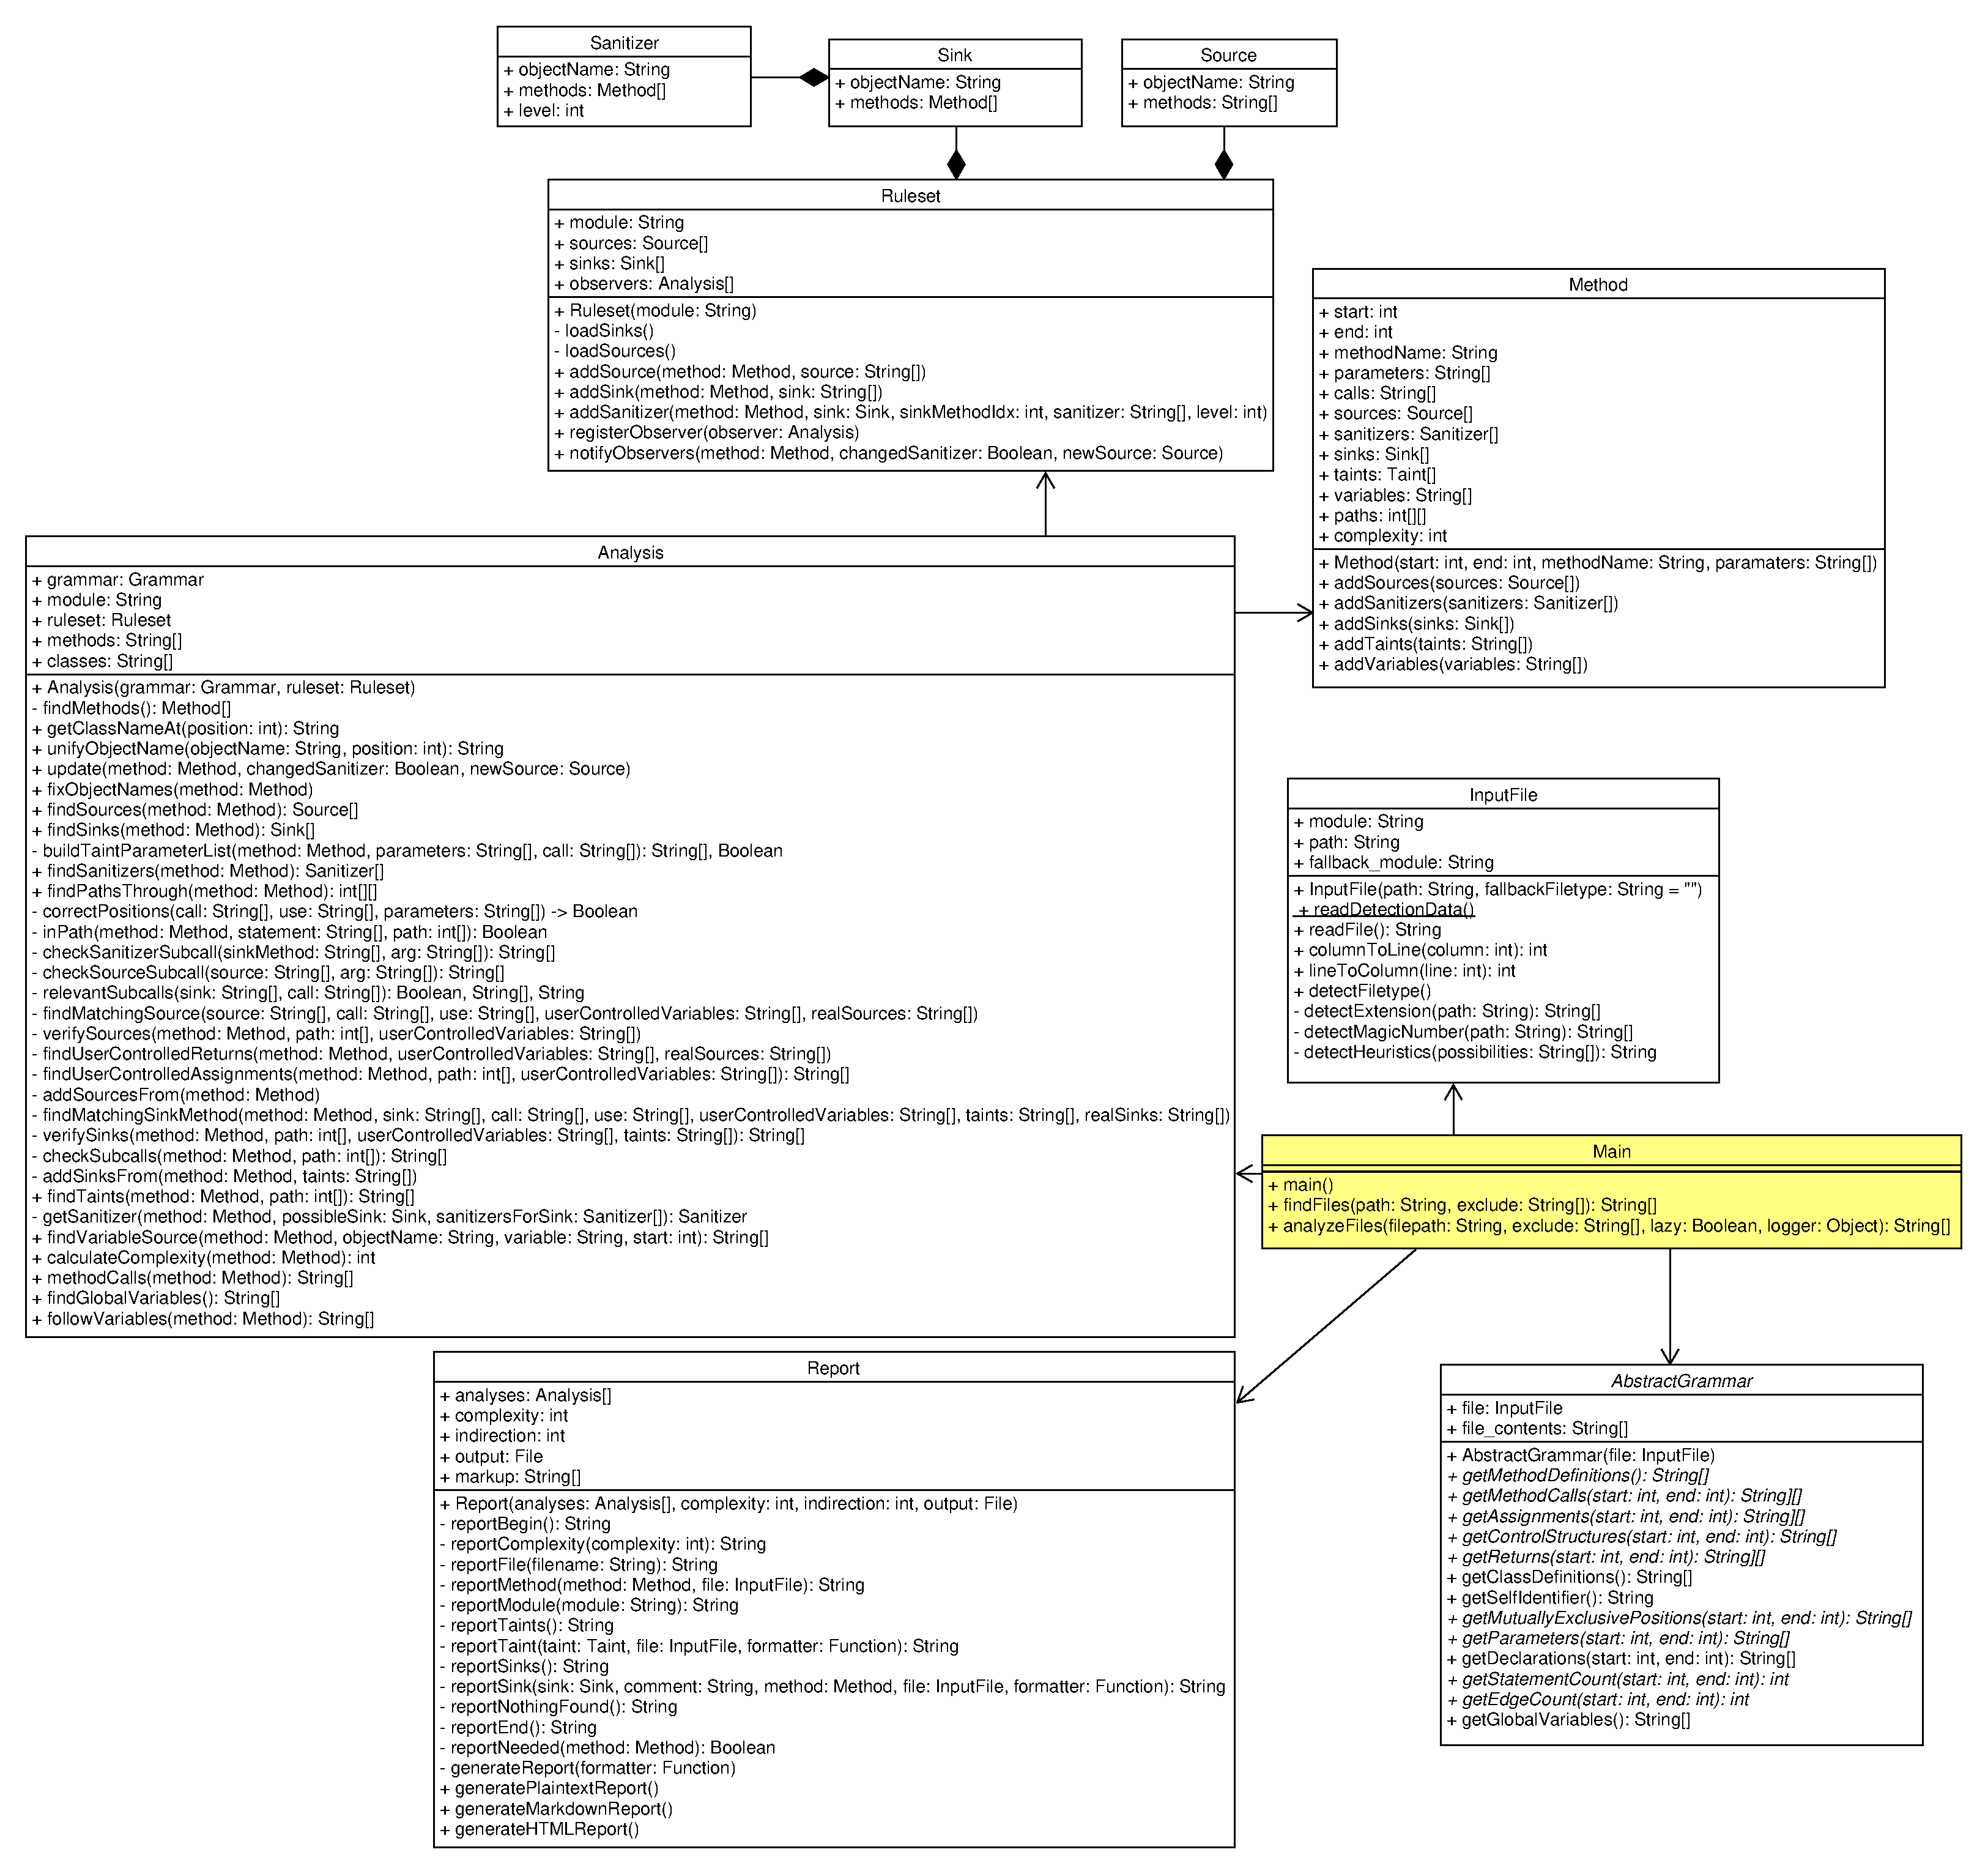
\includegraphics[max height=\textheight, max width=\columnwidth]{Klassendiagramm.pdf}
            \captionbelow{UML-Klassendiagramm des Frameworks}\label{fig:Klassendiagramm}
        \end{figure}

        Die Main"=Klasse wurde zur besseren Sichtbarkeit farbig hinterlegt.

        Nachdem in der Main"=Klasse die Kommandozeilenoptionen eingelesen und
        verarbeitet wurden
        (vergleiche
        \vref{Einlesen der Kommandozeilenoptionen}),
        werden die einzelnen Dateien eingelesen
        (vergleiche
        \vref{Einlesen der zu untersuchenden Quelltexte}) und
        deren Dateityp bestimmt
        (vergleiche
        \vref{Auswahl der Module für verschiedene Programmiersprachen}).

        Von dort aus werden die einzelnen Dateien durch den Parser für die Analyse vorbereitet
        (vergleiche
        \vref{Parsen der Quelltexte}),
        indem sie vom Parser in einen Parsetree,
        einen
        \gls{AST} und
        schließlich einen
        \gls{CFG} umgewandelt werden.

        Der resultierende
        \gls{CFG} kann dann analysiert werden,
        indem zuerst die passenden Regelsätze geladen werden
        (vergleiche
        \vref{Parsen der Regelsätze}) und
        anhand derer die Quellen,
        Senken und
        Absicherungen ermittelt werden
        (vergleiche
        \vref{Suche nach Schwachstellen}).

        Diese werden abgespeichert und
        später zur Generierung des Reports genutzt
        (vergleiche
        \vref{Erstellung eines Reports}).

        Der Report wird weiterhin um eine Analyse der Codekomplexität ergänzt
        (vergleiche
        \vref{Analyse der Codekomplexität}),
        wobei die Funktionen ausgegeben werden,
        deren zyklomatische Zahl einen bestimmten Grenzwert überschreiten.

    \section{Entwicklung in einer isolierten Umgebung}
        Da die Entwicklung des Frameworks in Python durchgeführt wird und
        verschiedene Abhängigkeiten genutzt werden,
        scheint es sinnvoll,
        die Entwicklung in einer isolierten Umgebung durchzuführen,
        um sicherzustellen,
        dass immer die passenden Bibliotheken genutzt werden und
        es zu keinen Problemen führt,
        wenn eine der Abhängigkeiten verändert wurde.

        In neueren Versionen von Python
        (ab 3.6) ist hierfür das Modul
        \lstinline{venv} in der Standardbibliothek enthalten,
        welches die Erstellung einer isolierten Umgebung erlaubt.

        \subsection{venv}
            \lstinline{venv} ist eine in den Standard aufgenommene Alternative zum verbreiteten
            \lstinline{Virtualenv} von Ian Bicking.\cite{Bicking2018}
            Es wird seit Python 3.3 offiziell als neuer Standard empfohlen.\cite{PSF2018c}

        \subsection{Pipenv}
            Obwohl die Nutzung einer virtuellen Umgebung mittels
            \lstinline{venv} bereits große Vorteile gegenüber einer Installation ohne isolierte Umgebung bietet,
            ist es trotzdem sinnvoll,
            zusätzlich zu
            \lstinline{venv} noch
            \lstinline{Pipenv} einzusetzen.

            Dies liegt daran,
            dass
            \lstinline{Pipenv} den Paketmanager
            \gls{PIP} und
            die isolierte Umgebung von
            \lstinline{venv} miteinander kombiniert und
            zusätzlich Hashes für sämtliche genutzten Pakete anlegt,
            durch welche zum einen die Installation deterministisch wird und
            zum anderen verhindert wird,
            dass Pakete manipuliert werden,
            sodass die Sicherheit erhöht wird,
            was insbesondere bei sicherheitskritischen Anwendungen wie
            einem statischen Codescanner wichtig ist.\cite{Reitz2018}

            Zur Installation werden Module daher hinzugefügt mit dem Befehl

            \begin{lstlisting}[caption={Hinzufügen neuer Module in Pipenv}, gobble=16]
                pipenv install PACKAGE
            \end{lstlisting}

            bzw. bei Paketen,
            welche nur für die Entwicklung notwendig sind und
            nicht für den späteren Produktiveinsatz

            \begin{lstlisting}[caption={Hinzufügen neuer Module in Pipenv}, gobble=16]
                pipenv install PACKAGE --dev
            \end{lstlisting}

            Nach Abschluss der Entwicklung werden sämtliche Abhängigkeiten und
            Dateihashes abgespeichert über

            \begin{lstlisting}[caption={Erstellung der Pipfile.lock}, gobble=16]
                pipenv lock
            \end{lstlisting}

            Skripte können ausgeführt werden mittels

            \begin{lstlisting}[caption={Ausführen von Skripten in Pipenv}, gobble=16]
                pipenv run COMMAND [ARGS] ...
            \end{lstlisting}

            Für die spätere Nutzung müssen Endanwender zuerst ebenfalls Pipenv installieren und
            dann mittels

            \begin{lstlisting}[caption={Installation der Pakete für Endanwender}, gobble=16]
                pipenv install --ignore-pipfile
            \end{lstlisting}

            die für die Laufzeit benötigten Pakete installieren.

            Um den Installationsprozess übersichtlich darzustellen,
            wurden sämtliche notwendigen Schritte in der Datei
            \filename{INSTALL.md} aufgelistet.

        \subsection{Erstellung eines Installationsskripts}
            Um die Installation des Frameworks zu vereinfachen,
            wurde ein Installationsskript angelegt.

            Durch dieses Skript wird zuerst
            \lstinline{Pipenv} auf dem System installiert und
            anschließend genutzt,
            um die Projektabhängigkeiten zu installieren.

            Hierdurch sollte es möglich sein,
            auf beliebigen Systemen mit installiertem Python 3 das Framework deterministisch zu installieren und
            auszuführen.

    \section{Codestil}
        Der Codestil orientiert sich an
        \gls{PEP} 8,
        dem offiziellen Styleguide von Python\cite{Rossum2013},
        sowie
        am Numpy Docstring Guide für Erklärungstexte in Modulen,
        Klassen und
        Funktionen.\cite{numpydocmaintainers2018}

        Obwohl Python eine dynamische Typisierung hat,
        werden durchgängig
        \foreignquote{english}{Type Hints} genutzt,
        welche andeuten,
        um was für einen Datentyp es sich handelt.\cite{Rossum2014}

        Da Type Hints allerdings nicht durch die Programmiersprache erzwungen werden,
        sind diese Hinweise vor allem für die bessere Lesbarkeit gedacht.

        Zusätzlich findet eine Codeprüfung mittels Flake8
        (\cite{Cordasco2018}) und
        Pylint
        (\cite{PyCQA}) statt,
        um einen sauberen und
        möglichst gut lesbaren Code sicherzustellen.

    \section{Unittests}
        Um die Funktionalität des Frameworks sicherzustellen und
        Regressionsfehler zu vermeiden,
        werden für alle wichtigen Funktionen des Frameworks Unittests erstellt,
        mithilfe derer Testeingaben mit zu erwartenden Ergebnissen verglichen werden.

        Hierdurch ist es möglich,
        Fehler in bestimmten Funktionen frühzeitig zu entdecken und
        sie zu beheben,
        damit es nicht zu Störungen im produktiven Betrieb kommt.

        Wie auch bei der statischen Analyse ist es allerdings unmöglich,
        mit Unittests den korrekten Ablauf eines Programms zu garantieren,
        sodass sie lediglich als zusätzliche Maßnahme zur Qualitätssicherung verwendet werden,
        statt als Garantie einer korrekten und
        fehlerfreien Funktion.

    \section{Einlesen der Kommandozeilenoptionen}\label{Einlesen der Kommandozeilenoptionen}
        Über die Kommandozeilenoptionen kann der Benutzer angeben,
        welche Funktionen des Frameworks er aufrufen möchte.

        Hierbei ist vor allem wichtig,
        dass der Nutzer einen Pfad angeben kann,
        in welchem die Dateien zu finden sind,
        welche durch das Framework untersucht werden sollen.

        Weitere Parameter sind optional und
        dienen der Konfiguration des Suchlaufs.

        So kann über den Parameter
        \lstinline{-i} oder
        \lstinline{--indirection} angegeben werden,
        ab wie vielen Stufen indirekten Aufrufs eine Absicherung nicht mehr als solche gewertet wird,
        da sie zu weit von der Senke entfernt ist.

        Der Parameter
        \lstinline{-c} oder
        \lstinline{--complexity} gibt an,
        wie komplex eine Funktion sein darf,
        bevor sie in den Report aufgenommen wird.
        Hierbei wird als Kennzahl die zyklomatische Zahl verwendet,
        mit den in
        \vref{Aussagekraft} beschriebenen Einschränkungen.

        Der Parameter
        \lstinline{-f} oder
        \lstinline{--filetype} kann genutzt werden,
        um die Erkennung eines Dateityps zu erzwingen,
        wenn keine automatische eindeutige Erkennung anhand der Dateiendung oder
        der magischen Zahl möglich ist.

        Der Parameter
        \lstinline{-o} oder
        \lstinline{--output} gibt eine Ausgabedatei für den Report an.
        Wenn der Parameter weggelassen wird,
        wird der Report im Textformat auf der Standardausgabe ausgegeben.
        Wird stattdessen eine Datei mit der Endung
        \lstinline{.markdown} oder
        \lstinline{.md} angegeben,
        wird der Report im Markdown"=Format ausgegeben oder
        bei einer Datei mit Endung
        \lstinline{.htm} oder
        \lstinline{.html} im
        \gls{HTML}"=Format und
        bei
        \lstinline{.txt} im Textformat.
        Abweichende Dateiendungen produzieren eine Warnung und
        eine Ausgabe im Textformat.

        \subsection{Erstellung einer Hilfe}
            Die eingebaute Programmhilfe,
            welche standardmäßig mit dem Parameter
            \lstinline{-h} oder
            \lstinline{--help} angezeigt wird,
            ist im
            \gls{POSIX}"=Format erstellt.\cite{OpenGroup2018}

            Hierdurch ist die Nutzung zum einen für erfahrenere Nutzer intuitiv möglich,
            da dieser Standard eine hohe Verbreitung hat,
            zum anderen ist es hiermit auch einfach möglich,
            die Optionen mittels
            \lstinline{docopt} zu parsen,
            welches
            -- anders als die sonst üblichen Standards
            \lstinline{optparse} und
            \lstinline{argparse}
            -- keine Hilfetexte basierend auf dem Code erstellt,
            sondern anhand des Hilfetextes selbstständig die Parameter erkennt.\cite{Keleshev2018}

        \subsection{Übergabe von Kommandozeilenoptionen mittels docopt}
            Durch die Nutzung von
            \lstinline{docopt} ist es möglich,
            Kommandozeilenoptionen direkt in der Hilfe des Programms zu definieren.

            Allerdings ist es hiermit nicht direkt möglich,
            auch die Korrektheit der Eingaben zu prüfen.

            Zu diesem Zweck wird
            \lstinline{docopt} im Framework mit
            \lstinline{schema} kombiniert.

            \lstinline{schema} ist ein Modul zur Validierung von Python"=Datenstrukturen,
            welches versucht,
            Daten in ein bestimmtes Format zu konvertieren.
            Wenn dies fehlschlägt,
            wird eine Fehlermeldung ausgegeben.\cite{Keleshev2018a}

    \section{Einlesen der zu untersuchenden Quelltexte}\label{Einlesen der zu untersuchenden Quelltexte}
        Um die zu untersuchenden Quelltexte einzulesen,
        wird die Python"=Funktion
        \lstinline{walk} eingesetzt,
        welche rekursiv Verzeichnisse durchläuft und
        dabei jeweils das aktuelle Verzeichnis,
        die enthaltenen Unterverzeichnisse und
        die enthaltenen Dateien zurückliefert.

        Da die Unterverzeichnisse selbst für dieses Framework nicht relevant sind,
        wird der zugehörige Wert ignoriert,
        was konventionsgemäß in Python durch einen Unterstrich ausgedrückt wird.

        Um hierbei nicht sämtliche Dateinamen gleichzeitig im Speicher halten zu müssen,
        wurde die Funktion zum Einlesen der Quelltexte als Generator geschrieben,
        was bedeutet,
        dass jeweils nur der aktuelle Wert zurückgegeben und
        die Funktion bei einem erneuten Aufruf an der Stelle fortgesetzt wird,
        wo die Ausführung beim letzten Mal durch das Schlüsselwort
        \lstinline{yield} unterbrochen wurde.

        Als Ergebnisse werden der
        (relative) Dateipfad und
        der Inhalt der Datei als Liste von Strings zurückgegeben.

    \section{Auswahl der Module für verschiedene Programmiersprachen}\label{Auswahl der Module für verschiedene Programmiersprachen}
        Um für jeden Quelltext die richtigen Regelsätze zu bestimmen,
        muss das Framework die Programmiersprache des Quelltextes korrekt erkennen und
        die zugehörigen Regelsätze laden.

        Da dieses Problem wie in
        \vref{Vergleich Dateiformaterkennung} beschrieben nicht ohne weiteres eindeutig lösbar ist,
        werden verschiedene Ansätze miteinander kombiniert.

        Zur Erkennung der Dateiformate wird im Unterverzeichnis
        \foreignquote{english}{modules} des Projekts eine Textdatei mit dem Namen
        \foreignquote{english}{detection.txt} benötigt.

        In dieser Datei steht,
        für welche Dateiendung und
        welche Erkennung durch die magische Zahl ein Modul ausgewählt werden sollte.

        Das Format ist hierbei so aufgebaut,
        dass zuerst das Modul,
        anschließend ein Doppelpunkt,
        dann die Dateiendungen mit vorangestelltem Punkt,
        getrennt durch Kommas und
        nach einem Semikolon der Anfang der Ausgabe des Magic"=Befehls steht.

        Zur Erläuterung soll das Beispiel aus
        \vref{lst:detection.txt} dienen.

        \begin{lstlisting}[caption={Beispieleinträge in der detection.txt}, label={lst:detection.txt}, gobble=12]
            c: .c, .h; C source
            cpp: .cc, .cpp, .hpp; C source
        \end{lstlisting}

        Wie man hieran sehen kann,
        kann es durchaus passieren,
        dass die Erkennung des Magic"=Befehls uneindeutig ist,
        weshalb zuerst die magische Zahl ermittelt wird und
        anschließend,
        wenn diese nicht eindeutig ist,
        die Ergebnisse durch die Dateiendung eingeschränkt werden.

        Sollte keine der beiden Methoden zu einem Ergebnis führen,
        so wird eine Heuristik basierend auf der Mehrheit der erkannten Dateiformate im aktuellen Verzeichnis eingesetzt,
        sofern der Anwender keine Rückfalllösung angegeben hat.

        \subsection{Erkennung des Dateiformats anhand der Endung}
            Um das Dateiformat anhand der Endung zu erkennen,
            wird die Funktion
            \lstinline{os.path.splitext} genutzt.

            Diese Funktion trennt den Dateinamen von der Erweiterung und
            gibt beides in einem Tupel zurück.

            Als Besonderheit gibt die Funktion bei Dateien,
            deren Namen mit einem Punkt beginnen und
            die keine eigene Dateierweiterung haben,
            den Dateinamen nicht als Erweiterung,
            sondern als Dateiname zurück,
            sodass zum Beispiel
            \lstinline{.bashrc} nicht als namenlose Datei mit der Endung
            \lstinline{.bashrc} erkannt wird,
            sondern als Datei mit dem Namen
            \lstinline{.bashrc} ohne Endung.

            Sämtliche passenden Module zu der gefundenen Dateiendung werden anschließend in einer Liste zurückgegeben.

        \subsection{Erkennung des Dateiformats mittels der magischen Zahl}
            Für die Erkennung mittels der magischen Zahl wird das Paket
            \lstinline{python-magic} verwendet,
            welches intern die Funktion des Unix"=Standardbefehls
            \lstinline{file} nachstellt.

            Da hierfür unter Windows zusätzliche Dateien benötigt werden,
            wurde ein Installationsskript für Windows erstellt,
            welches abhängig von der Architektur des Systems
            (32 Bit oder
            64 Bit) die entsprechenden Dateien aus einem Unterordner in das aktuelle Verzeichnis kopiert,
            damit sie von
            \lstinline{python-magic} gefunden werden können.

            Es ist hierbei wichtig zu erwähnen,
            dass durch die für die 32 Bit"=Version von Windows benötigte
            \gls{DLL} die Lizenz des kompletten Projekts von der sehr freien
            \gls{MIT}"=Lizenz auf die weit striktere
            \gls{GPL} wechselt,
            da ein wesentlicher Bestandteil nun unter
            \gls{GPL} steht.
            Alle weiteren verwendeten Bestandteile sind unter der
            \gls{MIT}"=Lizenz lizenziert,
            sodass diese auch für das Projekt verwendet werden könnte.

            Für die spätere Auslieferung könnte es daher sinnvoll sein,
            die Dateien für die 32 Bit"=Version von Windows nicht mitzuliefern und
            lediglich einen Hinweis auf die Quelle zu geben,
            damit die Anwender sie sich selbst beschaffen können.

            Da die Verbreitung von 32 Bit"=Windows"=Systemen ohnehin immer mehr abnimmt,
            sollte dies zu keinen großen Einschränkungen führen,
            erlaubt es allerdings,
            eine freiere Lizenz für das Gesamtprojekt zu wählen.

            Ebenso
            wie bei der Erkennung des Dateityps anhand der Erweiterung wird auch hier eine Liste von möglichen Modulen zurückgegeben.

        \subsection{Erkennung des Dateiformats anhand einer Heuristik}
            Um anhand der Heuristik ein Dateiformat zu erkennen,
            werden die anderen Dateien im gleichen Verzeichnis mittels der vorherigen Methoden ermittelt und
            anschließend das am häufigsten erkannte Dateiformat verwendet.

            Hierbei werden keine Unterordner durchsucht,
            da es vielfach üblich ist,
            Projektdateien,
            die in verschiedenen Programmiersprachen geschrieben sind,
            in unterschiedlichen Ordnern unterzubringen.

            Weiterhin kann eine Liste möglicher Dateiformate für die Heuristik übergeben werden,
            wenn die Erkennung zwar möglich,
            aber nicht eindeutig war.

            In diesem Fall wird die Liste der möglichen Module auf diese Module eingeschränkt,
            um eine Falscherkennung weiter zu minimieren.

            Sollte keine weitere Datei im gleichen Verzeichnis erkannt werden,
            so wird eine Warnung ausgegeben und
            die Datei bekommt kein Modul zugewiesen.

        \subsection{Erzwungene Erkennung unbekannter Dateiformate}
            Man kann der Klasse zur Behandlung von Eingabedateien einen String mitgeben,
            welcher ein Modul festlegt,
            welches genutzt werden soll,
            wenn die Erkennung anhand der Dateiendung und
            der magischen Zahl fehlschlägt.

            Wenn diese Funktion aktiviert wird,
            wird die Erkennung anhand der Heuristik automatisch deaktiviert.

            Sollte die Erkennung mittels der Dateiendung oder
            der magischen Zahl ein eindeutiges Ergebnis liefern,
            so wird dieses bevorzugt.

            Wenn die Erkennung mittels Dateiendung oder
            magischer Zahl kein eindeutiges Ergebnis zurückliefert,
            sondern eine Vielzahl von möglichen Erkennungen existiert,
            das erzwungene Modul aber nicht in dieser Liste enthalten ist,
            wird eine Warnmeldung ausgegeben.
            Die Erkennung wird allerdings trotzdem mit dem erzwungenen Modul durchgeführt.

        \subsection{Darstellung als Programmablaufplan}
            Der Algorithmus zur Erkennung des Dateiformats besteht aus mehreren Teilen,
            die miteinander zusammenarbeiten,
            um in möglichst vielen Fällen ein korrektes Ergebnis zu liefern.
            Ein vereinfachter Programmablaufplan des gesamten Algorithmus wie in
            \vref{fig:Erkennung_Dateiformat} kann die Zusammenhänge besser veranschaulichen.

            \begin{figure}[htp]
                \centering%
                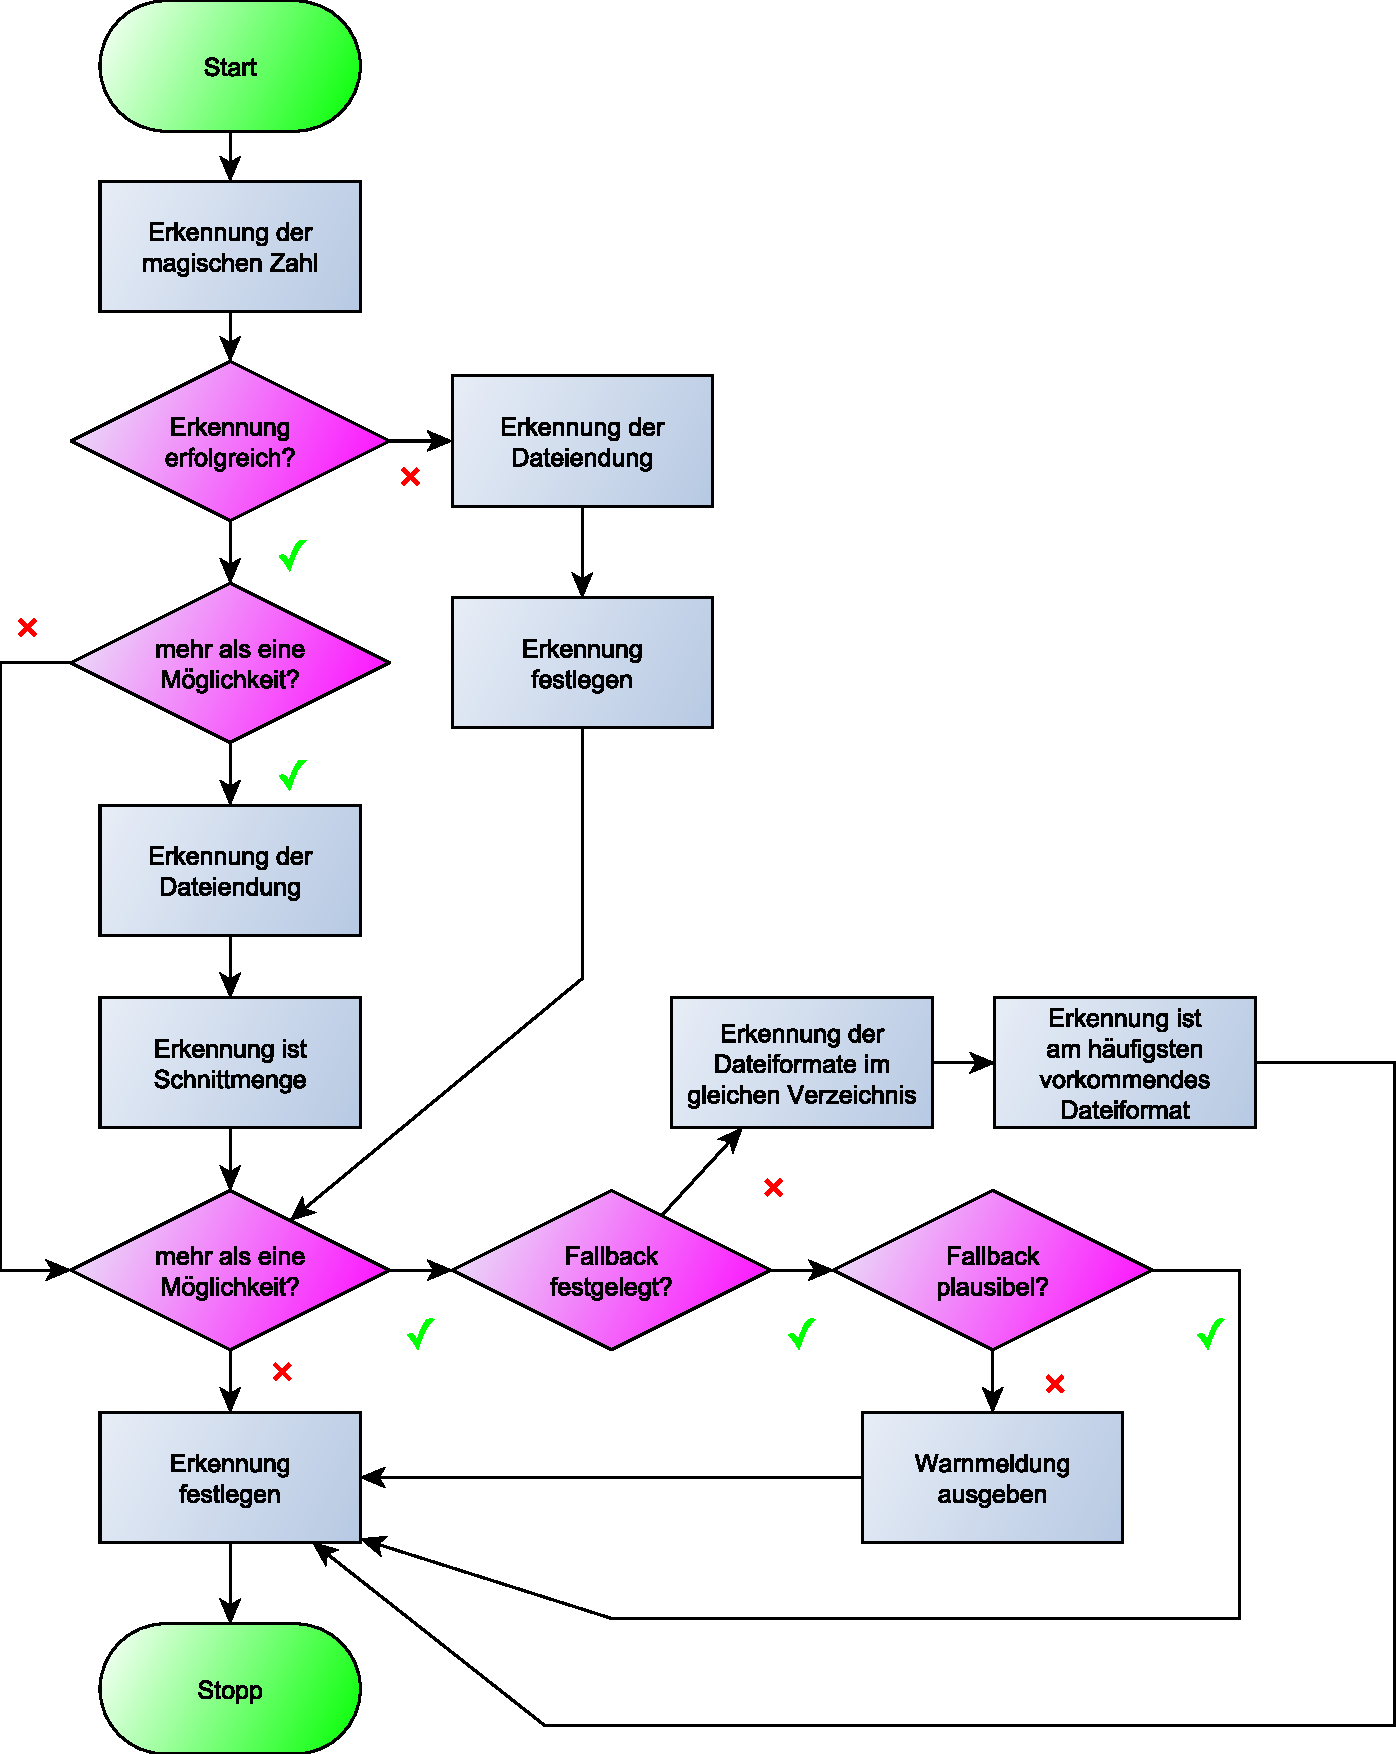
\includegraphics[max height=\textheight, max width=\columnwidth]{Erkennung_Dateiformat.pdf}
                \captionbelow{Gesamtalgorithmus zur Erkennung des Dateiformats}\label{fig:Erkennung_Dateiformat}
            \end{figure}

            Die Details sind den jeweiligen Unterabschnitten zu entnehmen.

    \section{Parsen der Quelltexte}\label{Parsen der Quelltexte}
        Um die Quelltexte auf Sicherheitslücken untersuchen zu können,
        müssen sie zuerst durch einen Parser in ein entsprechendes Format umgewandelt werden,
        indem
        wie in
        \vref{Aufbau eines Parsers} beschrieben für die Syntax unnötige Bestandteile entfernt und
        einzelne Bestandteile der Syntax mit ihrem Kontext extrahiert werden.

        Um den Parser zu realisieren,
        existieren in Python einige Bibliotheken,
        die jeweils ihre Vor"= und
        Nachteile haben und
        daher im Folgenden miteinander verglichen werden.

        Anschließend müssen die Grammatiken für die zu untersuchenden Sprachen erstellt werden,
        was ebenfalls exemplarisch vorgeführt wird,
        um späteren Benutzern eine Anleitung zu geben,
        wie sie eigene Grammatiken erstellen und
        warten können.

        Nachdem die Grammatiken erstellt wurden,
        werden sie genutzt,
        um Quelltexte einzulesen.
        Hierzu wird darauf eingegangen,
        in welcher Form sie schließlich für das Framework vorliegen und
        wie damit gearbeitet werden kann.

        Im letzten Schritt wird aus dieser Repräsentation ein
        \gls{AST} generiert,
        anhand dessen die eigentliche Schwachstellensuche durchgeführt wird.

        \subsection{Auswahl einer Bibliothek zum Parsen}
            In der Python"=Welt existieren viele verschiedene Bibliotheken,
            die es ermöglichen,
            einen Parser zu entwickeln.

            Da sich die Ziele dieser Bibliotheken allerdings teilweise erheblich unterscheiden,
            weil einige der Projekte mehr Wert auf die Geschwindigkeit beim Parsen,
            einige mehr auf die Mächtigkeit der Regelsätze und
            einige mehr auf die einfache Les"= und
            Schreibbarkeit legen,
            ist es wichtig,
            die Projekte miteinander zu vergleichen und
            ein Projekt zu finden,
            welches zum einen mächtig genug ist,
            um den Anforderungen dieser Masterarbeit zu genügen,
            zum anderen aber auch einfach genug in der Handhabung ist,
            dass es auch von späteren Anwendern weiterentwickelt und
            gewartet werden kann.

            Da sämtliche hier vorgestellten Bibliotheken entweder direkt unter der
            \gls{MIT}"=Lizenz stehen oder
            eine ähnlich freie Lizenz nutzen,
            bei der lediglich ein Hinweis auf die verwendete Bibliothek und
            die Lizenz vorhanden sein muss,
            hat die Lizenz der benutzten Bibliothek in diesem Fall keinen Einfluss auf die Lizenz des Frameworks.

            \subsubsection{PyParsing}
                PyParsing versucht,
                einen alternativen Ansatz zur üblichen Entwicklung von Grammatiken mit Lex und
                \gls{Yacc},
                zwei Standardwerkzeugen für die Compilerentwicklung,
                oder
                mittels regulärer Ausdrücken,
                zu schaffen.\cite{McGuire2018}

                PyParsing erlaubt es dabei,
                Grammatiken direkt in Python"=Code zu schreiben und
                versucht,
                eine gute Les"= und
                Schreibbarkeit zu ermöglichen,
                indem viele Hilfsklassen bereitgestellt werden,
                um die Compilerentwicklung zu beschleunigen.

                Die Nachteile von PyParsing sind,
                dass die Bibliothek vor allem auf einfache Grammatiken ausgelegt ist,
                die Performance bei komplexeren Grammatiken schlecht ist
                (\cite{McGuire2018a}) und
                die zu schreibende Grammatik sich nicht am Industriestandard Lex und
                \gls{Yacc} orientiert.

            \subsubsection{PLY}
                \gls{PLY} ist eine rein in Python geschriebene Reimplementierung von Lex und
                \gls{Yacc},
                welche sich vor allem durch eine gute Fehlerdiagnose auszeichnet.\cite{Beazley2018}

                Da sich
                \gls{PLY} stark am Industriestandard orientiert und
                gleichzeitig hilfreiche Fehlermeldungen ausgibt,
                ist es erfahrenen Compilerentwicklern möglich,
                vergleichsweise einfach einen Compiler in Python zu entwickeln.

                \gls{PLY} versucht dabei,
                schnell,
                speichereffizient und
                ausreichend mächtig für real existierende Programmiersprachen wie
                C,
                C++ oder
                Ada zu sein.\cite{Beazley2018}

                Als Nachteil von
                \gls{PLY} ist anzusehen,
                dass die Erstellung eines Parsers sehr aufwendig ist und
                stark auf regulären Ausdrücken beruht,
                welche als Docstrings von Methoden geschrieben werden,
                die durch eine spezielle Kennzeichnung im Modul von
                \gls{PLY} erkannt und
                interpretiert werden.

                Hierdurch ist es auch bei
                \gls{PLY} notwendig,
                die Eigenarten der Bibliothek zu lernen,
                um eigene Grammatiken zu erstellen.

                Außerdem ist es aufwendiger,
                vorhandene Grammatiken zu warten,
                da die Komplexität durch die starke Nutzung regulärer Ausdrücke schnell ansteigt,
                wie in
                \vref{fig:SQLi-Regex} im Grundlagenkapitel dargestellt.

            \subsubsection{SLY}
                \gls{SLY} ist eine Abwandlung von
                \gls{PLY},
                die aufgrund ihrer moderneren Implementierungsweise vom Autoren der beiden Bibliotheken empfohlen wird.\cite{Beazley2018}

                Die Syntax wurde gegenüber
                \gls{PLY} vereinfacht,
                da statt den Docstrings Dekorierer genutzt werden,
                anhand derer die Tokens innerhalb der Methoden interpretiert werden.

                \gls{SLY} hat allerdings den gleichen Nachteil
                wie
                \gls{PLY},
                dass die erstellten Grammatiken stark auf regulären Ausdrücken basieren,
                was die Wartbarkeit erschwert.

                Weiterhin ist das
                \gls{SLY}"=Projekt noch vergleichsweise jung,
                sodass nur wenige Beispiele und
                Anleitungen existieren,
                was die Erstellung eigener Grammatiken für Anwender maßgeblich erschwert.

            \subsubsection{Parsimonious}
                Parsimonious ist entstanden,
                um ein Problem von
                \gls{LALR(1)}"=Parsern,
                bei denen nur ein Token voraus geschaut werden kann,
                wie
                \gls{Yacc} zu lösen:
                uneindeutige Syntaxregeln.

                Als Beispiel beschreibt der Autor in einer Präsentation,
                dass er einen Link mit dem Format
                \lstinline{[[Titel|Link]]} parsen wollte.
                \gls{LALR(1)}"=Parser stießen in diesem Fall auf Probleme,
                wenn der Anfang des Textes zwar
                wie ein Link aussah,
                allerdings das Token zum Beenden des Links fehlte,
                wie im Beispiel von
                \lstinline{[[Titel|Link [[doch kein Link}.\cite{Rose2012}

                In diesem Fall sollte der Parser erkennen,
                dass es sich um keinen korrekten Link handelt und
                er entsprechend stattdessen den Text als normalen Text behandeln sollte.

                Da
                \gls{LALR(1)}"=Parser allerdings nur bis zum nächsten Token vorausschauen können,
                tritt in diesem Fall ein Fehler auf,
                da sie bereits die Erkennung als Link vorausgesetzt haben und
                jetzt keinen korrekten Link vorfinden.

                Parsimonious versucht weiterhin,
                ebenfalls gut les"= und
                schreibbare Grammatiken zu ermöglichen,
                indem es sich an einer vereinfachten
                \gls{EBNF} orientiert.

                Auch hier ist allerdings einer der Hauptnachteile,
                dass durch die starke Verwendung von regulären Ausdrücken die Wartbarkeit leidet.

            \subsubsection{Vergleich und Begründung der Entscheidung}\label{Vergleich und Begruendung der Entscheidung}
                Von den vorgestellten Bibliotheken scheint PyParsing am besten für die Zwecke dieses Frameworks geeignet zu sein.

                Dies liegt vor allem daran,
                dass es einfach ist,
                Grammatiken zu schreiben,
                sodass auch Anwender ohne Kenntnisse im Compilerbau in der Lage sind,
                Grammatiken für die von ihnen eingesetzten Sprachen zu erstellen,
                anstatt hoffen zu müssen,
                dass jemand anders diese Grammatiken für sie erstellt,
                oder
                die statische Analyse für diese Sprachen ausfallen zu lassen.

                Zwar ist PyParsing weniger mächtig,
                als die anderen vorgestellten Bibliotheken,
                allerdings ist es für das entwickelte Framework bereits ausreichend,
                wenn die Definition von Modulen,
                Objekten und
                Funktionen sowie
                der Aufruf dieser und
                Zuweisungen korrekt erkannt werden können,
                um Schwachstellen zu erkennen.

                Eine komplette Grammatik,
                mit welcher der gesamte Quelltext untersucht werden kann,
                ist zum einen sehr aufwendig zu erstellen,
                zum anderen allerdings auch weniger robust,
                da in anderen Versionen der Programmiersprache die Syntax geändert sein kann,
                wodurch die erstellte Grammatik nicht mehr fehlerfrei durchläuft.

                Wie in
                \vref{Problemstellung und
                -abgrenzung} beschrieben,
                ist es weiterhin nicht Ziel des Frameworks,
                die korrekte Syntax eines Quelltextes sicherzustellen,
                sodass es einfacher ist,
                zu versuchen,
                nur die relevanten Teile des Quelltextes zu parsen und
                die restlichen Teile zu ignorieren.

                Diese Entscheidung bedeutet allerdings nicht,
                dass Anwender nicht auch die Möglichkeit haben,
                andere Bibliotheken zum Parsen der Quelltexte zu verwenden.

                Stattdessen erlaubt es das Design über die abstrakte Basisklasse
                \lstinline{AbstractGrammar},
                beliebigen eigenen Code zu verwenden,
                um die Grammatik für den Parser zu implementieren,
                solange die entsprechenden Methoden der Basisklasse implementiert sind und
                die erwarteten Rückgabewerte haben.

                Hiermit wird wieder eines der Hauptziele des Frameworks,
                eine möglichst hohe Flexibilität für den Endanwender,
                gefördert.

                Im nächsten Unterabschnitt wird jedoch nur auf die Erstellung von Grammatiken mittels PyParsing eingegangen,
                da dies
                wie oben erwähnt am realistischsten der Situation für Endanwender entspricht.

        \subsection{Erstellung der Grammatiken}
            Um aufzuzeigen,
            wie einfach es ist,
            eine neue Grammatik für das Framework zu schreiben,
            wird im Folgenden beispielhaft erläutert,
            wie die Grammatik zum Parsen von C"=Quelltexten erstellt wurde.

            Es ist hierbei wichtig zu beachten,
            dass keine vollständige Grammatik erstellt wird,
            sondern nur die für die spätere Schwachstellenerkennung notwendigen Bestandteile aufgenommen werden.

            Eine derartige unvollständige Grammatik hat dabei einige Vorteile,
            aber auch einige Nachteile gegenüber vollständigen Grammatiken.

            Zum einen sind unvollständige Grammatiken weitaus schneller zu erstellen,
            als vollständige,
            da viele Bestandteile weggelassen werden können,
            was auch die Wartung vereinfacht.

            Außerdem sind unvollständige Grammatiken robuster gegenüber Änderungen in der Syntax der Programmiersprache,
            da neue syntaktische Möglichkeiten nicht zum Abbruch des Parsens führen,
            sondern einfach überlesen und
            ignoriert werden.

            Für die Zwecke dieses Frameworks ist es dabei nur erforderlich,
            Zuweisungen,
            Funktionsdeklarationen,
            Funktionsaufrufe sowie
            Rückgabewerte korrekt zu erkennen,
            um somit analysieren zu können,
            wie der Kontrollfluss des Programms aussieht und
            ob es hierbei zu Schwachstellen kommen könnte.

            Auf der anderen Seite haben unvollständige Grammatiken den Nachteil,
            dass es hiermit schwieriger ist,
            die Codekomplexität mittels der in
            \vref{Berechnung der McCabe-Metrik} vorgestellten McCabe"=Metrik zu bestimmen,
            da
            wie oben erwähnt Kontrollstrukturen nicht unbedingt erkannt werden.

            Es bietet sich daher an,
            eine Art Pseudoerkennung für Kontrollstrukturen einzuführen,
            bei der lediglich ein zu der Kontrollstruktur gehöriges Schlüsselwort gesucht wird und
            die Anzahl der Treffer gezählt wird.

            \subsubsection{Erstellung einer unvollständigen Grammatik für C}
                Im Folgenden wird erklärt,
                wie vorgegangen werden kann,
                um mittels PyParsing eine unvollständige Grammatik für C"=Programme zu erstellen.

                Zwar ist es
                wie in
                \vref{Vergleich und Begruendung der Entscheidung} auch möglich,
                beliebige andere Bibliotheken zu benutzen,
                um eine Grammatik zu erstellen,
                jedoch wird PyParsing als einfache und
                mächtige Alternative aufgezeigt,
                um zu demonstrieren,
                dass es hiermit problemlos möglich ist,
                Grammatiken für eigene,
                bisher noch nicht vom Framework unterstützte Programmiersprachen zu erstellen.

                Selbstverständlich kann im Folgenden keine vollständige Anleitung zur Erstellung eines Parsers mit PyParsing erstellt werden,
                es wird allerdings versucht,
                auf einige unter Umständen verwirrende oder
                uneindeutige Konstrukte hinzuweisen und
                sie zu erklären sowie
                eine Grundlage zu schaffen,
                anhand derer Endanwender unter Zuhilfenahme der bisherigen Grammatiken sowie
                der offiziellen Dokumentation unter
                \cite{McGuire2018a} schnell in der Lage sein sollten,
                eigene Grammatiken zu erstellen.

                Das Programm zum Erstellen der Grammatik muss dabei im Verzeichnis
                \filename{modules} innerhalb des gewünschten Moduls als
                \filename{grammar.py} erstellt werden.

                Um eine grobe Struktur vorzugeben,
                ist es sinnvoll,
                von der zuvor bereits erwähnten abstrakten Oberklasse
                \lstinline{AbstractGrammar} zu erben,
                welche die vom Framework erwarteten Methoden enthält.

                Der Konstruktor der Klasse sollte als Eingabe ein
                \lstinline{InputFile}"=Objekt erwarten,
                welches an den Konstruktor der Oberklasse weitergereicht wird.

                Anschließend kann die eigentliche Beschreibung der Grammatik erfolgen.

                Es bietet sich an,
                hierbei möglichst viele Hilfsstrukturen zu erstellen,
                um eine einfache Erweiterbarkeit und
                die größtmögliche Übersichtlichkeit zu gewährleisten.

                So könnte als Erkennung für eigene Bezeichnungen für Variablen und
                Funktionen in C Folgendes genutzt werden:

                \begin{lstlisting}[caption={Erkennung von Bezeichnungen in C}, gobble=20, language=python]
                    self.ident = Word(alphas, alphanums + "_")
                \end{lstlisting}

                Hierdurch werden Wörter erkannt,
                welche mit einem Buchstaben beginnen und
                anschließend eine Kombination aus Buchstaben,
                Zahlen und
                dem Unterstrich haben.

                Diese Erkennung kann anschließend weiterverwendet werden,
                zum Beispiel bei der Erkennung von Variablentypen.

                \begin{lstlisting}[caption={Erkennung von Variablentypen}, gobble=20, language=python]
                    self.vartype = Suppress(Combine(Optional(oneOf("signed " \
                                                                   "unsigned")) +
                                                    self.ident +
                                                    Optional(Word("*")),
                                                    adjacent=False))
                \end{lstlisting}

                In dieser Erkennung werden die Variablentypen mittels
                \lstinline{Suppress} unterdrückt,
                da sie für die Erkennung von Schwachstellen nicht relevant sind.

                Anschließend werden Variablentypen definiert als eine Kombination von einem optionalen Schlüsselwort
                \lstinline{signed} oder
                \lstinline{unsigned},
                dem eben definierten Erkennungstypen für Bezeichnungen und
                schließlich einem oder
                mehreren Sternen,
                welche die Variable als Zeiger identifizieren.

                Um die Grammatik
                später im Programm einfacher verarbeiten zu können,
                können nach den Tokendefinitionen Bezeichnungen hinzugefügt werden,
                wodurch es
                später im Code möglich ist,
                per Schlüsselwort auf das Token zuzugreifen,
                indem in Klammern nach der Definition ein Bezeichner eingetragen wird.

                Der Schlüsselwortparameter
                \lstinline{adjacent} der
                \lstinline{Combine}"=Klasse wird dabei auf
                \lstinline{False} gesetzt,
                um dafür zu sorgen,
                dass Leerzeichen zwischen den einzelnen Tokens nicht die Erkennung verhindern.

                Eine weitere wichtige Eigenheit von PyParsing sind die sogenannten Forward"=Deklarationen.

                Da es sich bei PyParsing um einen Recursive Descent"=Parser handelt,
                kann es vorkommen,
                dass Tokens verwendet werden,
                welche zum Zeitpunkt der Verwendung noch nicht definiert sind.

                Um dieses Problem zu beheben,
                können diese Tokens mittels
                \lstinline{Forward()} definiert und
                im späteren Verlauf mit Erkennungen befüllt werden.

                Als Beispiel hierfür soll die Deklaration von Funktionskörpern dienen,
                bei denen es notwendig ist,
                Statements und
                Funktionsprototypen vorab zu definieren,
                die allerdings zu diesem Zeitpunkt in der Grammatik noch nicht existieren.

                \begin{lstlisting}[caption={Definition der Erkennung von Funktionskörpern}, gobble=20, language=python]
                    self.stmt = Forward()
                    self.prototype = Forward()
                    self.func_body = Group(
                        OneOrMore(Group(SkipTo(self.stmt, failOn=self.prototype,
                                               include=True))))
                \end{lstlisting}

                Wie hier zu sehen ist,
                werden Funktionskörper definiert als eine Gruppe aus einer oder
                mehreren Gruppen,
                welche wiederum aus Statements bestehen.

                Um zu erreichen,
                dass der Parser nicht abstürzt,
                wenn er auf einen unbekannten Token stößt,
                wird hierbei die
                \lstinline{SkipTo}"=Klasse verwendet,
                welche so lange Tokens liest und
                direkt verwirft,
                bis sie ein weiteres Statement erreicht.

                Wenn
                \lstinline{SkipTo} dabei über einen Funktionsprototypen läuft,
                wird die Rekursion an dieser Stelle beendet und
                der Prototyp wird nicht in die Erkennung aufgenommen.

                Der Schlüsselwortparameter
                \lstinline{include} führt hierbei dazu,
                dass der Parser die unbekannten Tokens nicht einfach überliest,
                sondern auch die Auswertung des Quelltextes erst nach den übersprungenen Tokens weiter fortsetzt.

                Um schließlich die Forward"=Deklarationen mit Erkennungsmustern zu befüllen,
                wird mittels
                \lstinline{<<} im späteren Programm der Inhalt festgelegt.

                \begin{lstlisting}[caption={Befüllen einer Forward-Deklaration}, gobble=20, language=python]
                    self.stmt << (self.func_call("func_call") |
                                  self.assignment("assignment") |
                                  self.return_("return")) + Suppress(";")
                \end{lstlisting}

                Nachdem sämtliche benötigten Strukturen und
                Tokens definiert wurden,
                müssen noch einige Methoden erstellt werden,
                welche von der
                \lstinline{AbstractGrammar} vorgegeben wurden und
                im späteren Programm für die Auswertung genutzt werden.

                Da diese Methoden beliebige Abschnitte der Quelltexte durchsuchen können sollen,
                sollte die Funktion
                \lstinline{scanString} der jeweiligen Tokendefinition genutzt werden,
                durch welche das Parsen nicht unbedingt am ersten Zeichen der Eingabe starten muss,
                sondern beliebige Zeichen am Anfang überliest,
                bis die korrekte Eingabe gefunden wurde.

                Es kann weiterhin sinnvoll sein,
                vor dem Beginn des Parsens mittels
                \lstinline{ParserElement.enablePackrat()} das sogenannte Packrat"=Parsing zu aktivieren,
                wodurch Ergebnisse des Parsevorgangs memoisiert werden,
                was zu einer deutlichen Performancesteigerung bei umfangreicheren Quelltexten führen kann.

                Sollte die eigene Grammatik allerdings Parseraktionen durchführen,
                welche in PyParsing dazu dienen,
                das Ergebnis des Parsevorgangs direkt weiterzuverarbeiten,
                so könnten sich durch Packrat schwer auffindbare Fehler ergeben.

                Da Parseraktionen allerdings in den bisher erstellten Grammatiken nie notwendig waren,
                werden sie hier nicht näher besprochen und
                das Aktivieren von Packrat wird empfohlen.

        \subsection{Repräsentation im Programm}
            Um die Ergebnisse des Parsers im Programm darzustellen,
            wird von PyParsing eine eigene Datenstruktur verwendet,
            auf welche man wie eine Kombination aus Listen und
            Hashmaps
            (in Python als
            \foreignquote{english}{Dictionaries} bezeichnet)
            zugreifen kann.

            Die Listen enthalten dabei die erkannten Tokens,
            denen keine Bezeichnung zugeordnet wurde,
            die Dictionaries dagegen enthalten als Schlüssel die Bezeichnung und
            als Wert das Token.

            So kann man in der folgenden Auswertung einer C"=Funktion sowohl
            über den Index,
            also mittels
            \lstinline{parsetree[0][0]},
            auf den Funktionsnamen zugreifen als auch über die Bezeichnung,
            also mittels
            \lstinline{parsetree[0]['name']}.

            \begin{lstlisting}[caption={Repräsentation einer einfachen C-Funktion}, gobble=16, language=python]
                ((['add',
                    (['a'], {'name': ['a']}),
                    (['b'], {'name': ['b']}),
                    ([(['', 'c', (['a', 'b'], {})],
                    {'lvalue': ['c'],
                        'expression': [(['a', 'b'], {})],
                        'assignment': [(['c', (['a', 'b'], {})], {})]}),
                    (['', 'c'], {'return_value': ['c'], 'return': [(['c'], {})]})],
                    {})],
                    {'name': ['add'],
                    'args': [([(['a'], {'name': ['a']}), (['b'], {'name': ['b']})], {})],
                    'body': [([(['', 'c', (['a', 'b'], {})],
                        {'lvalue': ['c'],
                        'expression': [(['a', 'b'], {})],
                        'assignment': [(['c', (['a', 'b'], {})], {})]}),
                    (['', 'c'], {'return_value': ['c'], 'return': [(['c'], {})]})],
                    {})]}),
                    0,
                    58)
            \end{lstlisting}

            Dies erleichtert die spätere Auswertung ungemein,
            da es möglich ist,
            mittels einfacher Abfragen zu untersuchen,
            ob ein Token an einer bestimmten Stelle im Parsetree existiert.

            Die verwendeten Bezeichnungen für die Tokens müssen dabei einheitlich sein,
            damit bei der späteren Analyse auf sie zurückgegriffen werden kann.

            Es ist daher sinnvoll,
            sich bei der Erstellung neuer Grammatiken nach Möglichkeit an bestehenden Grammatiken zu orientieren und
            auch deren Bezeichnungen zu übernehmen,
            um ein gutes Ergebnis zu erzielen.

            Sollten die Bezeichnungen fehlen,
            kann das Framework im Nachhinein nicht mehr identifizieren,
            um welches Token es sich handelt,
            und
            kann daher keine Schwachstellenanalyse durchführen.

            Die beiden Zahlen am Ende geben an,
            in welcher Spalte der Funktionsbeginn bzw.\ das Funktionsende erkannt wurden.

            Wenn andere Bibliotheken zur Erstellung der Grammatiken benutzt werden sollen,
            müssten deren Ergebnisse so umgewandelt werden,
            dass sie mit der hier vorliegenden Form kompatibel sind,
            bevor sie vom Framework verwendet werden können.

            Da Python Duck"=Typing einsetzt,
            ist es hierbei lediglich erforderlich,
            dass die Ergebnisse sich anhand der Bezeichner und
            Listenindizes zuordnen lassen und
            die zugehörigen Angaben zur Start"= und
            Endposition im String in einer Liste an der zweiten,
            bzw.\ dritten Stelle auftauchen,
            um eine Kompatibilität mit dem restlichen Framework zu gewährleisten.

        \subsection{Analyse des AST}
            Für die Analyse des
            \gls{AST} werden in der Klasse
            \lstinline{AbstractGrammar} einige abstrakte und
            auch konkrete Methoden vorgegeben,
            welche helfen,
            relevante Informationen aus dem Parsetree zu extrahieren.

            Bei den abstrakten Methoden handelt es sich zum Beispiel um
            \lstinline{getMethodDefinitions()},
            welche sämtliche Methoden innerhalb einer Datei zurückgibt,
            \lstinline{getMethodCalls(start, end)},
            welche sämtliche Methodenaufrufe zwischen zwei Spalten der Eingabe zurückgibt,
            \lstinline{getAssignments(start, end)},
            welche alle Zuweisungen zwischen zwei Spalten der Eingabe zurückgibt und
            \lstinline{getReturns(start, end)},
            welche alle Rückgabewerte einer Methode zurückgibt.

            Diese Methoden müssen von der jeweiligen Grammatik konkret implementiert werden und
            werden von den folgenden konkreten Methoden verwendet,
            um eine Analyse des Datenflusses zu ermöglichen.

            In der Analyse"=Klasse werden diese Methoden dann benutzt.

            \lstinline{followVariables(method)} gibt eine Übersicht über die Zuweisungen und
            Funktionsaufrufe,
            in welchen Variablen verwendet werden.

            Um den Ursprung der Variablen zurückzuverfolgen,
            kann
            \lstinline{findVariableSource(method, objectName, variable, start)} verwendet werden,
            wodurch Variablen ab der Position
            \lstinline{start} zurück zur letzten Zuweisung innerhalb der gleichen Methode verfolgt werden.

            Durch diese Funktionen ist es möglich,
            nachzuvollziehen,
            wie sich Variablen im Code ausbreiten und
            damit herauszufinden,
            ob eine Verunreinigung möglich ist.

    \section{Parsen der Regelsätze}\label{Parsen der Regelsätze}
        Die Regelsätze werden wie
        in
        \vref{Vergleich der Formate und Auswahl} beschrieben in
        \gls{YAML} geschrieben und
        in Python mittels PyYAML ausgewertet.

        Hierzu ist es zuerst wichtig,
        zu entscheiden,
        für welches Modul die Regelsätze geladen werden sollen.

        Für diese Entscheidung dient das Ergebnis aus
        \vref{Auswahl der Module für verschiedene Programmiersprachen},
        welches der Regelsatzklasse
        \lstinline{Ruleset} im Konstruktor mitgegeben wird.

        Anhand dieses Moduls werden anschließend die Regeln für Senken und
        deren zugehörige Bereinigungen sowie
        die Regeln für die Quellen geladen.

        Um dies zu erreichen,
        werden alle Dateien mit den Endungen
        \lstinline{.yaml} oder
        \lstinline{.yml} im Unterverzeichnis
        \lstinline{modules/MODULE/sinks} bzw.
        \lstinline{modules/MODULE/sources} mittels PyYAML ausgelesen.

        Hierbei wird,
        aus den in
        \vref{YAML} beschriebenen Gründen,
        die Methode
        \lstinline{yaml.safe_load} eingesetzt,
        um Code Execution durch bösartige Regeln zu verhindern.

        Das Ergebnis wird anschließend an die entsprechenden Klassen für die Repräsentation der einzelnen Regeln übergeben.

        \subsection{Definition von Schwachstellen}
            Für die Definition einer Schwachstelle mit den zugehörigen Absicherungen wird die Klasse
            \lstinline{Sink} eingesetzt.

            Diese prüft zunächst den Objektnamen aus der
            \gls{YAML}"=Regel,
            wobei wie in
            \vref{Vergleich der beiden Ansätze} beschrieben jeweils nur ein Objekt pro Regeldatei beschrieben wird,
            sodass der erste Eintrag des übergebenen Dictionaries als Objektname erkannt wird.

            Im Anschluss kann auf die Methoden über den Schlüssel
            \lstinline{Methods} zugegriffen werden.

            Um auch die Absicherungen von einem Dictionary in Objekte der Klasse
            \lstinline{Sanitizer} zu übertragen,
            ist es erforderlich,
            zuerst den Originaleintrag zwischenzuspeichern und
            anschließend aus den Einträgen zu den Absicherungen jeweils
            \lstinline{Sanitizer}"=Objekte zu erstellen,
            welche die Dictionary"=Einträge überschreiben.

            Um schließlich sicherzustellen,
            dass auch die weiteren Inhalte der Regeldatei existieren,
            werden Assertions eingesetzt,
            welche mithilfe der Python"=Funktion
            \lstinline{all()} und
            List Comprehension,
            einer kompakten Technik zur Erzeugung von Listen,
            prüfen,
            ob alle Methoden ebenfalls einen
            \lstinline{Methodname},
            \lstinline{Parameters} und
            \lstinline{Comment} enthalten.

            Da diese Assertions unter Umständen bei einer Vielzahl von Regelsätzen die Ausführung ein wenig verlangsamen können,
            ist es möglich,
            diese entweder mittels
            \lstinline{pipenv run python -O main.py} oder
            mittels der Umgebungsvariable
            \lstinline{PYTHONOPTIMIZE=TRUE} zu deaktivieren.

            In diesem Fall könnte es allerdings passieren,
            dass im späteren Verlauf der Ausführung Fehler auftreten,
            sodass diese Option nur genutzt werden sollte,
            wenn die Performance des Frameworks problematisch ist.

        \subsection{Definition von Sicherungen}
            Die Definition von Sicherungen erfolgt ebenso wie die Definition von Schwachstellen,
            indem der erste Schlüssel im übergebenen Dictionary als Objektname und
            dessen Methoden als
            \lstinline{Methods} erkannt werden.

            Auch hier werden Assertions eingesetzt,
            um das Format der Regeldatei zu überprüfen,
            die wie oben beschrieben deaktiviert werden können.

        \subsection{Definition benutzerkontrollierter Eingaben}
            Auch die Definition benutzerkontrollierter Eingaben verhält sich analog zu der Definition von Sicherungen,
            da auch diese Klasse lediglich der einfacheren Datenhaltung dient.

            Ebenso wie in den Schwachstellen und
            Sicherungen werden auch hier Assertions eingesetzt,
            um das Format zu prüfen.

    \section{Suche nach Schwachstellen}\label{Suche nach Schwachstellen}
        Um Schwachstellen zu erkennen,
        werden in der Analyse zuerst alle Klassen und
        Methoden der Eingabedatei erkannt.

        Anschließend wird eine Datenflussanalyse durchgeführt,
        bei der versucht wird,
        sämtliche Verwendungen von Variablen zurückzuverfolgen und
        somit aufzulisten,
        an welcher Stelle welche Variable eingesetzt wird.

        Die Liste der Variablen wird dabei mit allen Verwendungen abgespeichert und
        für alle weiteren Analyseschritte verwendet.

        Da es bei der objektorientierten Programmierung allerdings vorkommen kann,
        dass Variablennamen mehrdeutig sind,
        müssen anschließend die Objektbezeichnungen innerhalb der Variablenliste angeglichen werden.

        Als Beispiel hierfür seien die Schlüsselwörter
        \lstinline{this} in Java oder
        \lstinline{self} in Python genannt.

        Diese beiden Schlüsselwörter deuten an,
        dass der Kontext der referenzierten Variable die aktuell umgebende Klasse ist.

        Wenn nun die Analyse versucht,
        eine Verwendung dieser Variablen in anderen Klassen zu suchen,
        muss zuerst die Selbstreferenz aufgelöst und
        durch den passenden Klassennamen ersetzt werden.

        Ferner müssen für manche Sprachen,
        wie Python,
        teilweise noch die Dateinamen als optionaler Teil des Objektnamens vorangestellt werden,
        da ein Zugriff auch über den Modulnamen möglich ist,
        welcher standardmäßig dem Dateinamen entspricht.

        Eine derartige Angleichung der Objektnamen würde zwar die Interpretation der Anweisung ändern,
        da das Framework allerdings eine rein statische Analyse durchführt,
        ist dies die einzige Möglichkeit,
        Methoden und
        Variablen auch über mehrere Klassen hinweg zuverlässig zu erkennen.

        Nachdem sämtliche Variablen gefunden und
        vereinheitlicht wurden,
        kann begonnen werden,
        mithilfe der Regelsätze nach Schwachstellen in den Quelltexten zu suchen.

        Um diese Regelsätze allerdings dynamisch erweitern zu können,
        da zum Beispiel der Aufruf einer Senke mit Parametern,
        welche von den Parametern der aufrufenden Methode abhängen,
        die aufrufende Methode selbst wiederum zu einer Senke macht,
        sind zwei Entwurfsmuster notwendig,
        welche im Folgenden kurz erklärt werden sollen:
        Das Observer"=Pattern und
        Dependency Injection.

        \subsection{Das Observer-Pattern}
            Um eine dynamische Erweiterung der Regelsätze zu ermöglichen,
            muss die Analyse nach jeder Änderung einer Regel erneut durchgeführt werden,
            um sicherzustellen,
            dass auch die neuen Regeln während des Suchlaufs beachtet werden.

            Um dies zu bewerkstelligen,
            wird im Framework eine einfache Variante des Observer"=Patterns eingesetzt.

            Beim Observer"=Pattern gibt es ein zu beobachtendes Objekt und
            mehrere Beobachter,
            die über Änderungen am Objekt informiert werden müssen.

            \begin{figure}[htp]
                \centering%
                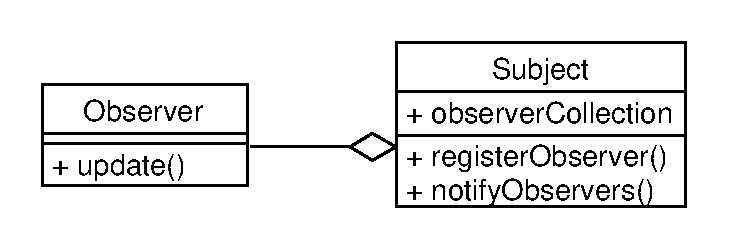
\includegraphics[max height=\textheight, max width=\columnwidth]{Observer-Pattern.pdf}
                \captionbelow{Einfache Form des Observer-Patterns}\label{fig:Observer-Pattern}
            \end{figure}

            Das Prinzip wird in
            \vref{fig:Observer-Pattern} veranschaulicht.

            Das zu beobachtende Objekt erhält eine Sammlung von Observern,
            welche über Änderungen am internen Zustand informiert werden sollen.

            Zu diesem Zweck müssen sich die Observer bei ihrer Erstellung mittels der Funktion
            \lstinline{registerObserver()} beim Subjekt registrieren.

            Sobald sich der interne Zustand des Subjekts ändert,
            müssen nun die Observer mittels
            \lstinline{notifyObservers()} darüber informiert werden,
            indem auf jedem Observer in der
            \lstinline{observerCollection} die Funktion
            \lstinline{update()} aufgerufen wird.

            Es gibt dabei verschiedene Varianten des Observer"=Patterns.
            Für das Framework wurde eine Push"=Variante gewählt,
            bei welcher der
            \lstinline{update()}"=Funktion der Observer direkt die geänderten Daten mitgegeben werden.

            Weiterhin wurde auf Funktionen zum Löschen von Observern verzichtet,
            da es hierfür keinen Bedarf gibt,
            auch wenn diese Funktion im Pattern eigentlich enthalten ist.

        \subsection{Dependency Injection}
            Ein weiteres Problem,
            welches durch die dynamischen Regelsätze bedingt ist,
            besteht darin,
            dass die Regelsätze nicht mehrfach instantiiert werden dürfen,
            da es ansonsten möglich ist,
            dass ein Objekt eines Regelsatzes nicht alle neu hinzugefügten Regeln enthält und
            somit eine unvollständige Analyse durchführt.

            Um dieses Problem zu beheben,
            wurde Dependency Injection eingesetzt.

            Bei Dependency Injection werden einem Objekt die Abhängigkeiten eines anderen Objekts mitgeliefert,
            sodass es sich seine Abhängigkeiten nicht mehr selbst suchen muss.

            Im konkreten Fall erwartet der Konstruktor der Analyseklasse eine zusätzliche Referenz auf seinen zu nutzenden Regelsatz,
            sodass es möglich ist,
            die Regelsätze einmalig für alle benötigten Programmiersprachen zu initialisieren und
            anschließend diese bereits initialisierten Regelsätze in die Analyse weiterzugeben,
            anstatt zu versuchen,
            aus der Analyse heraus selbst den passenden Regelsatz zu finden.

            Eine Alternative zur Dependency Injection wäre es zwar gewesen,
            ein Singleton"=,
            bzw.\ in diesem Fall ein Multiton"=Pattern einzusetzen,
            da Regelsätze für verschiedene Module möglich sind,
            allerdings werden Singletons häufig als Anti"=Pattern bezeichnet,\cite{Hevery2008}
            da sie wie versteckte globale Variablen agieren und
            somit den Code und
            das Testen schwerer verständlich machen.

        \subsection{Ablauf eines Suchdurchlaufs}
            Beim ersten Suchdurchlauf werden alle potenziell interessanten Funktionen abgespeichert,
            die als Senken,
            Quellen oder
            Absicherungen fungieren könnten.

            Im ersten Schritt wird dabei nach Quellen gesucht,
            indem geprüft wird,
            welche Funktionsaufrufe sich innerhalb der aktuellen Methode befinden.

            Wenn eine Funktion gefunden wird,
            deren Bezeichnung und
            Parameteranzahl zu einer der Regeln aus den Regelsätzen passt,
            wird der Funktionsaufruf als potenzielle Quelle in der Methode abgespeichert.

            Nach dem gleichen Prinzip können auch die Senken einer Methode ermittelt werden.

            Bei den Absicherungen dagegen ist es notwendig,
            die Absicherungen jeder einzelnen Senke zu suchen,
            da die Absicherungen direkt von den Senken abhängig sind.

            Wichtig ist hierbei,
            dass bei keiner der Prüfungen sofort sicher ist,
            ob sie wirklich eine der oben genannten Funktionen haben oder
            nicht.
            Dies liegt daran,
            dass zu diesem Zeitpunkt noch nicht überprüft werden kann,
            ob die Parameter der Funktionen benutzerkontrolliert sind oder
            nicht,
            da diese Funktion erst bei der Suche nach Verschmutzungen zum Einsatz kommt.

            Globale Variablen werden immer wie zusätzliche Parameter einer Funktion behandelt und
            somit als potenziell benutzerkontrolliert angesehen,
            da es nicht möglich ist,
            die Veränderung dieser Werte in einer statischen Analyse vorherzusagen.

            \subsubsection{Notwendigkeit der erneuten Prüfung und Suche nach Verschmutzungen}
                Zur Suche nach Verschmutzungen müssen die gefundenen potenziell interessanten Funktionen erneut überprüft werden,
                da es nun möglich ist,
                deren Parameter mit einer Liste von benutzerkontrollierten Variablen zu vergleichen.

                Hierzu müssen zuerst die vom Benutzer potenziell kontrollierbaren Variablen ermittelt werden,
                also die Parameter der Funktion,
                Variablen,
                welche in Quellen verwendet werden,
                und
                Zuweisungen von benutzerkontrollierten Variablen an neue Variablen.

                Im Anschluss können dann diese bekanntermaßen durch den Benutzer kontrollierten Variablen genutzt werden,
                um zu prüfen,
                ob die Parameter einer Senke wirklich durch einen Benutzer kontrolliert werden oder
                nicht.

                Sollten benutzerkontrollierte Eingaben in eine Senke einfließen,
                so muss geprüft werden,
                ob die entstandene Verschmutzung vor der Nutzung abgesichert wurde.

                Da die Absicherung allerdings wie in
                \vref{Definition von Absicherungen} beschrieben niemals als 100\,\%ige Sicherheit angesehen werden sollte,
                wird die Absicherung lediglich als zusätzliche Information an die Verschmutzung angehängt.

                Im Anschluss daran wird die Senke zur Liste der
                \enquote{echten} Senken hinzugefügt,
                selbst wenn keine Benutzereingabe hierfür erkannt wurde,
                da noch immer die Möglichkeit besteht,
                dass die Benutzereingabe lediglich nicht durch die Regelsätze erfasst wurde.

                Dies ist erneut ein Versuch,
                eine maximale Erkennung zu gewährleisten und
                lieber zu viel zu erkennen,
                als Sicherheitslücken unentdeckt zu lassen.

                Wenn dagegen sicher ist,
                dass es sich um eine Verschmutzung handelt,
                die Senke also mit benutzerkontrollierten Daten befüllt wird,
                so wird versucht zu erkennen,
                von welchen Parametern der Methode die Parameter der Senke abhängig sind,
                und
                die Methode selbst mit ihren Parametern,
                welche an den Stellen,
                an denen sie in die Parameter der Senke einfließen,
                durch
                \command{\$TAINT} ersetzt werden,
                als neue Senke aufgenommen,
                wenn alle Parameter der Senke durch die Parameter der Methode beeinflusst werden.

                Es ist hierbei wichtig,
                dass nicht nur geprüft wird,
                ob ein Parameter der Methode von der Senke abhängig ist,
                sondern ob alle Parameter der Senke von denen der Methode abhängen,
                da die Regelsätze so konzipiert sind,
                dass Benutzer für den Fall,
                dass es egal ist,
                ob Parameter A oder
                Parameter B einer Senke benutzerkontrolliert ist,
                zwei einzelne Regeln erstellen sollten,
                bei denen jeweils einer der Parameter kontrolliert wird,
                sowie
                bei Bedarf eine weitere zusätzliche Regel für den Fall,
                dass beide Parameter kontrolliert werden sollen.

            \subsubsection{Generierung des Kontrollflussgraphen}
                Die Generierung des Kontrollflussgraphen ergibt sich aus mehreren Bestandteilen.

                Zum einen wird bei der Erkennung der Variablen und
                Methodenaufrufe abgespeichert,
                an welcher Position sich die jeweiligen Treffer befinden.

                Zum anderen wird eine Funktion namens
                \lstinline{find_variable_source()} genutzt,
                welche in der Lage ist,
                anhand eines Variablennamens und
                einer Startposition alle Zuweisungen dieser Variable an andere Variablen zu erkennen und
                somit rekursiv herauszufinden,
                was die ursprüngliche Quelle der Variable war.

                Als Beispiel soll im Folgenden versucht werden,
                die ursprüngliche Quelle der Variable
                \lstinline{test} herauszufinden,
                welche in Zeile 7 genutzt wird.

                \begin{lstlisting}[caption={Beispiel für eine Variablenrückverfolgung}, label={lst:Variablenrückverfolgung}, gobble=20]
                    #include <stdio.h>

                    int main(int argc, char * argv[]) {
                        char * foo = argv[1];
                        char * bar = foo;
                        char * test = bar;
                        printf(test);
                    }
                \end{lstlisting}

                Um nun herauszufinden,
                ob die Variable
                \lstinline{test} von einer Benutzereingabe beeinflusst wird,
                muss die Variable an der Startposition in Zeile 7,
                dem Aufruf der
                \lstinline{printf}"=Funktion,
                zurückverfolgt werden.

                Hierfür wird zuerst rückwärts nach der ersten Zuweisung gesucht,
                welche der Variable einen neuen Wert zuweist,
                da diese Zuweisung den Wert der Variable überschreibt.

                Erkannt wird hierdurch die Variable
                \lstinline{bar} in Zeile 6,
                sodass die Verfolgung nun rekursiv weitergeht und
                versucht,
                den Ursprung der Variable
                \lstinline{bar} zu erkennen.

                Auch hier wird wieder rückwärts nach der ersten Zuweisung gesucht und
                die Zuweisung von
                \lstinline{foo} an
                \lstinline{bar} in Zeile 5 entdeckt.

                Die Rekursion startet daher erneut und
                findet die Zuweisung von
                \lstinline|argv[1]| an
                \lstinline{foo} in Zeile 4.

                \lstinline{argv} wiederum wird anschließend als Parameter der Funktion in Zeile 3 erkannt und
                es ergibt sich ein Verlauf von
                \lstinline{argv}
                \textrightarrow{}
                \lstinline{foo}
                \textrightarrow{}
                \lstinline{bar}
                \textrightarrow{}
                \lstinline{test},
                die Variable ist also benutzerkontrolliert.

                Zusammen mit den anderen Informationen über die Positionen von Variablen und
                Methodenaufrufen ergeben sich hiermit alle vom Framework für den Kontrollflussgraphen benötigten Informationen.

            \subsubsection{Exklusive Kontrollstrukturen}
                Der Kontrollflussgraph kann sich weiterhin ändern,
                indem Kontrollstrukturen benutzt werden,
                welche sich gegenseitig ausschließen.

                Zu diesem Zweck wird im Folgenden der Begriff der
                \definition{exklusiven Kontrollstruktur} eingeführt,
                womit solche Kontrollstrukturen gemeint sind,
                bei denen es nur möglich ist,
                jeweils eine ihrer Alternativen zu durchlaufen,
                aber niemals mehrere.

                Das bekannteste Beispiel hierfür sind Bedingungen mittels
                \lstinline{if},
                \lstinline{if else} und
                \lstinline{else},
                wobei es bei jedem Durchlauf nur möglich ist,
                entweder in den
                \lstinline{if}"= oder
                in den
                \lstinline{if else}"= oder
                in den
                \lstinline{else}"=Zweig zu gehen,
                aber niemals in mehr als einen gleichzeitig.

                Auf der anderen Seite erlauben
                \definition{inklusive Kontrollstrukturen} wie
                \lstinline{for} oder
                \lstinline{while},
                dass das Programm sowohl in die Schleife wechselt,
                als auch anschließend den danach stehenden Code ausführt,
                auch wenn es nicht zwingend notwendig ist,
                dass die Schleife überhaupt durchlaufen wird.

                Diese verschiedenen Pfade durch eine Methode werden vom Framework mittels der Methode
                \lstinline{find_paths_through} erkannt und
                können anschließend getrennt voneinander durchlaufen werden,
                um zu verhindern,
                dass eine Quelle innerhalb einer Bedingung als Verschmutzung für eine Senke im Alternativblock erkannt wird.

        \subsection{Speicherung der Suchergebnisse}
            Die Suchergebnisse werden in Objekten für die untersuchten Methoden selbst abgespeichert.

            Dabei werden sowohl die Start"= und
            Endposition der Methode,
            der Methodenname und
            die Parameter als auch sämtliche Funktionsaufrufe und
            Variablen sowie
            alle Quellen,
            Senken,
            Absicherungen und
            Verschmutzungen mit abgespeichert,
            um zum Beispiel eine mehrfache Suche nach allen Variablen oder
            Funktionsaufrufen,
            die sich während der Analyse nicht ändern,
            zu verhindern.

            Da es weiterhin möglich ist,
            neue Quellen,
            Senken,
            Absicherungen oder
            Verschmutzungen hinzuzufügen,
            existieren Methoden,
            um die bisherigen Treffer zu erweitern.

            Ein Entfernen dieser Informationen ist dagegen nicht vorgesehen,
            weshalb sie entweder komplett ersetzt oder
            mit den entsprechenden Methoden ergänzt werden müssen.

    \section{Analyse der Codekomplexität}\label{Analyse der Codekomplexität}
        Für die Analyse der Codekomplexität wird wie in
        \vref{Berechnung der McCabe-Metrik} beschrieben die McCabe"=Metrik eingesetzt.

        Um die Berechnung durchzuführen,
        wird die Anzahl der Knoten und
        der Kanten bestimmt und
        anschließend wie zuvor angegeben miteinander verrechnet.

        Da die Bestimmung von Kanten und
        Knoten abhängig von der jeweiligen Sprache ist,
        muss deren Bestimmung in den einzelnen Grammatiken stattfinden.

        Hierbei ist wichtig zu beachten,
        dass unterschiedliche Typen von Kontrollstrukturen zu einer unterschiedlichen Anzahl möglicher Kanten führen.

        So führt eine Schleife zum Beispiel zu insgesamt drei Kanten,
        da sowohl der Schritt vom Start der Schleife zur ersten Anweisung innerhalb des Schleifenrumpfs,
        als auch der Schritt vom Start der Schleife zur Anweisung nach der Schleife,
        wenn sie nicht
        (mehr) durchlaufen wird,
        als auch der Schritt vom Ende des Schleifenrumpfs zurück zum Schleifenkopf betrachtet werden müssen.

        Auf der anderen Seite können exklusive Kontrollstrukturen die Anzahl der Kanten nur um jeweils zwei Kanten erhöhen,
        da sie definitionsgemäß entweder betreten werden können oder
        nicht.

        \subsection{Einschränkungen der Komplexitätsprüfung}
            Die Komplexitätsprüfung ist dadurch eingeschränkt,
            dass die korrekte Berechnung der Komplexität in hohem Maß abhängig von der Implementierung innerhalb der Grammatik ist.

            Es ist leider nicht möglich,
            hier eine feste Vorgabe zu machen,
            ohne den Erstellern zukünftiger Grammatiken vorzuschreiben,
            mit welcher Methode und
            welchen Bezeichnungen ihre eigenen Grammatiken erstellt werden müssen.

            Da es allerdings das Ziel des Frameworks ist,
            eine einfache Erweiterung durch Benutzer zu ermöglichen,
            sodass Benutzer auch selbst innerhalb kurzer Zeit noch nicht existierende Grammatiken erstellen können,
            kann nicht immer gewährleistet werden,
            dass die Berechnung der Komplexität in jedem Fall das korrekte Ergebnis bringt.

    \section{Erstellung eines Reports}\label{Erstellung eines Reports}
        Um die Ausgaben des Frameworks sinnvoll auswerten zu können,
        ist es notwendig,
        diese ein wenig aufzubereiten.

        Zu diesem Zweck kann das Framework Reports in drei verschiedenen Formaten erstellen:
        Als reine Textdatei,
        als Markdown"=Datei sowie
        als
        \gls{HTML}"=Datei.

        Diese Reports sind darauf ausgelegt,
        nicht mehr den Fortschritt oder
        Informationen zum Programmablauf innerhalb des Frameworks zu vermitteln,
        sondern in einer übersichtlichen Form auf mögliche Probleme innerhalb der analysierten Dateien hinzuweisen.

        Zu diesem Zweck wird eine private Methode,
        \lstinline{generate_report},
        innerhalb der
        \lstinline{Report}"=Klasse eingesetzt,
        welche eine generische Aufbereitung der Analyseresultate vornimmt.

        Hierfür werden Funktionen eingesetzt,
        die passende Textstücke zurückgeben und
        wo nötig vorher die benötigten Informationen aus den gespeicherten Ergebnissen extrahieren.

        Die Methode
        \lstinline{generate_report} formatiert weiterhin sämtliche Ausgaben,
        indem vor und
        nach jedem Textbaustein ein Markup eingefügt wird und
        die Textbausteine mit einer übergebenen Funktion formatiert werden.

        Hierdurch ist es möglich,
        fast beliebige Markup"=Formate zu implementieren,
        indem lediglich das Markup angepasst und
        eine passende Formatierungsfunktion implementiert bzw.\ angegeben wird.

        Damit der Report weiß,
        welche Ergebnisse er wo ausgeben muss,
        müssen ihm die Analyseergebnisse als Liste,
        die maximale zyklomatische Komplexität,
        die maximale Entfernung zwischen der Senke und
        der Absicherung sowie
        der Ausgabestrom mitgegeben werden.

        \subsection{Erstellung eines Reports als Textdatei}
            Die Erstellung des Reports als Textdatei ist die einfachste Variante,
            da es hierbei lediglich notwendig ist,
            die
            \lstinline{generate_report}"=Funktion mit den Standardparametern aufzurufen,
            wodurch eine Textdatei ohne jegliche Auszeichnungen erstellt wird.

        \subsection{Erstellung eines Reports als Markdown-Datei}
            Für die Erstellung des Markdown"=Reports müssen zuerst die Markupinformationen angepasst werden,
            indem die entsprechenden Einträge in der Klassenvariable
            \lstinline{markup} überschrieben werden.

            Anschließend wird auch hier wieder die
            \lstinline{generate_report}"=Funktion genutzt,
            welche die passende Ausgabe generiert.

        \subsection{Erstellung eines Reports als HTML-Datei}
            Für die Erstellung des Reports als
            \gls{HTML}"=Datei müssen ebenfalls die Markupinformationen angepasst werden.

            Um allerdings hierbei noch eine weitere Formatierung nach Corporate Identity Standards durchzuführen,
            werden zusätzlich die Datei
            \filename{style.css} und
            \filename{logo.png} eingebunden,
            mit welchen Endanwender den Report an ein für sie passendes Design anpassen können.

            Weiterhin wird das JavaScript
            \filename{customize.js} eingebunden,
            mit welchem weitere Anpassungen möglich sind.

            Um zu verhindern,
            dass durch die Nutzung von Sonderzeichen in den analysierten Dateien Probleme bei der Anzeige auftreten,
            werden sämtliche Ausgaben mittels
            \lstinline{html.escape} formatiert,
            um Sonderzeichen zu filtern.
